% BLAKE2 hashing [RFC 7693, §3.3]: h_0 is the IV XORed with the parameter block; the data
% blocks d_0 ... d_{dd-1} (the zero-padded key block, if any, then the zero-padded message) are
% compressed in order with the byte counter t; the last block has the final flag set; the digest
% is the first nn bytes of the final chain value.
% Original drawing for the Hash library.
\documentclass[tikz,border=6pt]{standalone}
\usepackage[T1]{fontenc}
\usepackage{lmodern}
% Shared style for the Hash diagrams.
% Palette: Okabe–Ito (colour-blind safe). Every diagram is drawn on an opaque white card so it
% stays legible on dark page themes.
\usetikzlibrary{arrows.meta,positioning,calc,fit,backgrounds}
\definecolor{hsblue}{HTML}{0072B2}
\definecolor{hsorange}{HTML}{E69F00}
\definecolor{hsgreen}{HTML}{009E73}
\definecolor{hsvermilion}{HTML}{D55E00}
\definecolor{hspurple}{HTML}{CC79A7}
\definecolor{hsink}{HTML}{1F2933}
\tikzset{
  >={Stealth[length=2.2mm]},
  every node/.style={font=\sffamily\small, text=hsink},
  wire/.style={draw=hsink, line width=0.6pt, ->},
  reg/.style={draw=hsink, line width=0.6pt, fill=hsblue!12, minimum width=9mm, minimum height=7mm},
  fn/.style={draw=hsink, line width=0.6pt, fill=hsorange!25, rounded corners=2pt, minimum width=10mm, minimum height=6mm},
  input/.style={draw=hsink, line width=0.6pt, fill=hsgreen!20, minimum width=9mm, minimum height=6mm},
  add/.style={circle, draw=hsink, line width=0.6pt, fill=white, inner sep=0pt, minimum size=5mm, font=\sffamily\bfseries},
  card/.style={fill=white, rounded corners=4pt},
}

\begin{document}
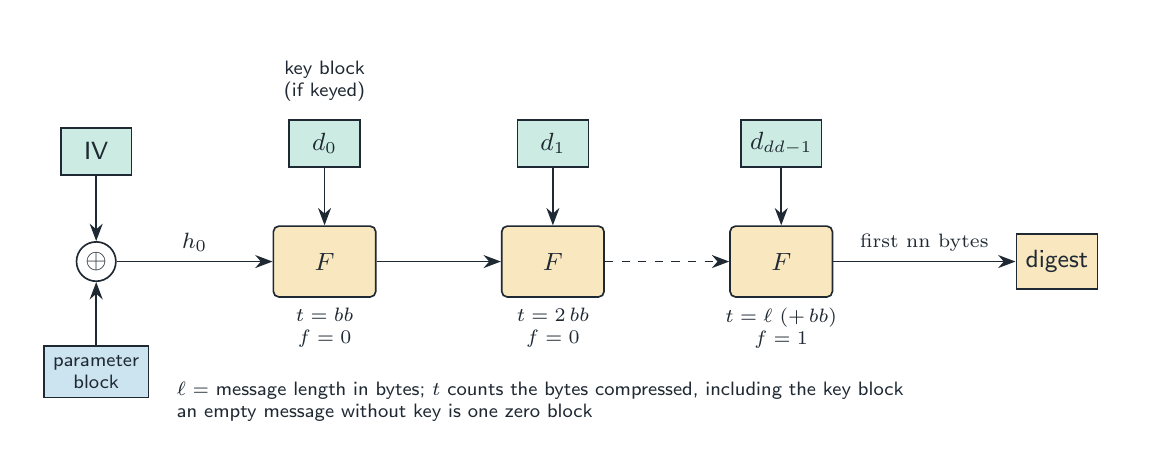
\begin{tikzpicture}
  \def\dx{2.9}
  \node[input, fill=hsgreen!20] (IV) at (0,1.4) {IV};
  \node[input, fill=hsblue!20, align=center, font=\sffamily\scriptsize] (PB) at (0,-1.4)
    {parameter\\block};
  \node[add] (x0) at (0,0) {$\oplus$};
  \draw[wire] (IV) -- (x0);
  \draw[wire] (PB) -- (x0);
  \foreach \i/\lbl/\t/\f in {1/{d_0}/{t = bb}/0, 2/{d_1}/{t = 2\,bb}/0, 3/{d_{dd-1}}/{t = \ell\ (+\,bb)}/1} {
    \node[fn, minimum width=13mm, minimum height=9mm] (F\i) at (\i*\dx, 0) {$F$};
    \node[input] (D\i) at (\i*\dx, 1.5) {$\lbl$};
    \draw[wire] (D\i) -- (F\i);
    \node[font=\sffamily\scriptsize, anchor=north, align=center] at (F\i.south)
      {$\t$\\$f = \f$};
  }
  \draw[wire] (x0) -- node[above, font=\footnotesize] {$h_0$} (F1);
  \draw[wire] (F1) -- (F2);
  \draw[wire, dashed] (F2) -- (F3);
  \node[reg, fill=hsorange!25] (out) at (4*\dx + 0.6, 0) {digest};
  \draw[wire] (F3) -- node[above, font=\scriptsize] {first nn bytes} (out);
  \node[font=\sffamily\scriptsize, anchor=south, align=center] at ($(D1.north)+(0,0.1)$)
    {key block\\(if keyed)};
  \node[font=\sffamily\scriptsize, anchor=north west, align=left] at (0.9,-1.4)
    {$\ell$ = message length in bytes; $t$ counts the bytes compressed, including the key block\\
     an empty message without key is one zero block};
  \begin{scope}[on background layer]
    \coordinate (e1) at (-0.8,-2.3);
    \coordinate (e2) at (4*\dx+1.4,2.9);
    \node[card, fit=(e1)(e2), inner sep=2pt] {};
  \end{scope}
\end{tikzpicture}
\end{document}
